\chapter{Background and Related Work} \label{Chap2}

% ############################################################################
\section{North Wyke Farm Platform and Eddy Covariance Measurement}

% ############################################################################
\subsection{Experimental Design and Management Regimes}

The North Wyke Farm Platform (NWFP), operated by Rothamsted Research near
Okehampton in Devon, UK, is a farm-scale National Bioscience Research
Infrastructure established in 2010 to investigate the productivity and
environmental sustainability of temperate livestock and arable farming
systems. The platform covers approximately 63~ha and comprises three outdoor
experimental systems, known as the Red, Green, and Blue farmlets, each
covering approximately 21~ha. Each farmlet contains five hydrologically
isolated catchments, giving 15 catchments across the platform in total.
Catchments may comprise either a single field or multiple separately managed
fields. They are hydrologically isolated through the combined effects of local
topography, slowly permeable subsoils, and a 9.2-km network of French drains
that directs runoff towards instrumented flumes
\cite{hawkins2023design,hawkins2025}.

The three farmlets represent contrasting agricultural management systems. The Red farmlet operates 
as an arable system with crop rotations including wheat, oats, and field beans. The Green farmlet 
represents a conventional permanent-pasture system, supporting seasonal cattle and sheep grazing 
alongside silage production and inorganic fertiliser application. The Blue farmlet combines high-sugar 
perennial ryegrass with white clover, supporting outdoor livestock production while using biological 
nitrogen fixation to reduce reliance on inorganic nitrogen fertiliser. Together, the farmlets allow 
arable, permanent-pasture, and grass--clover livestock systems to be studied under the same wider 
environmental setting \cite{hawkins2023design,hawkins2023fieldevents}.

\begin{figure}[htbp]
    \centering
    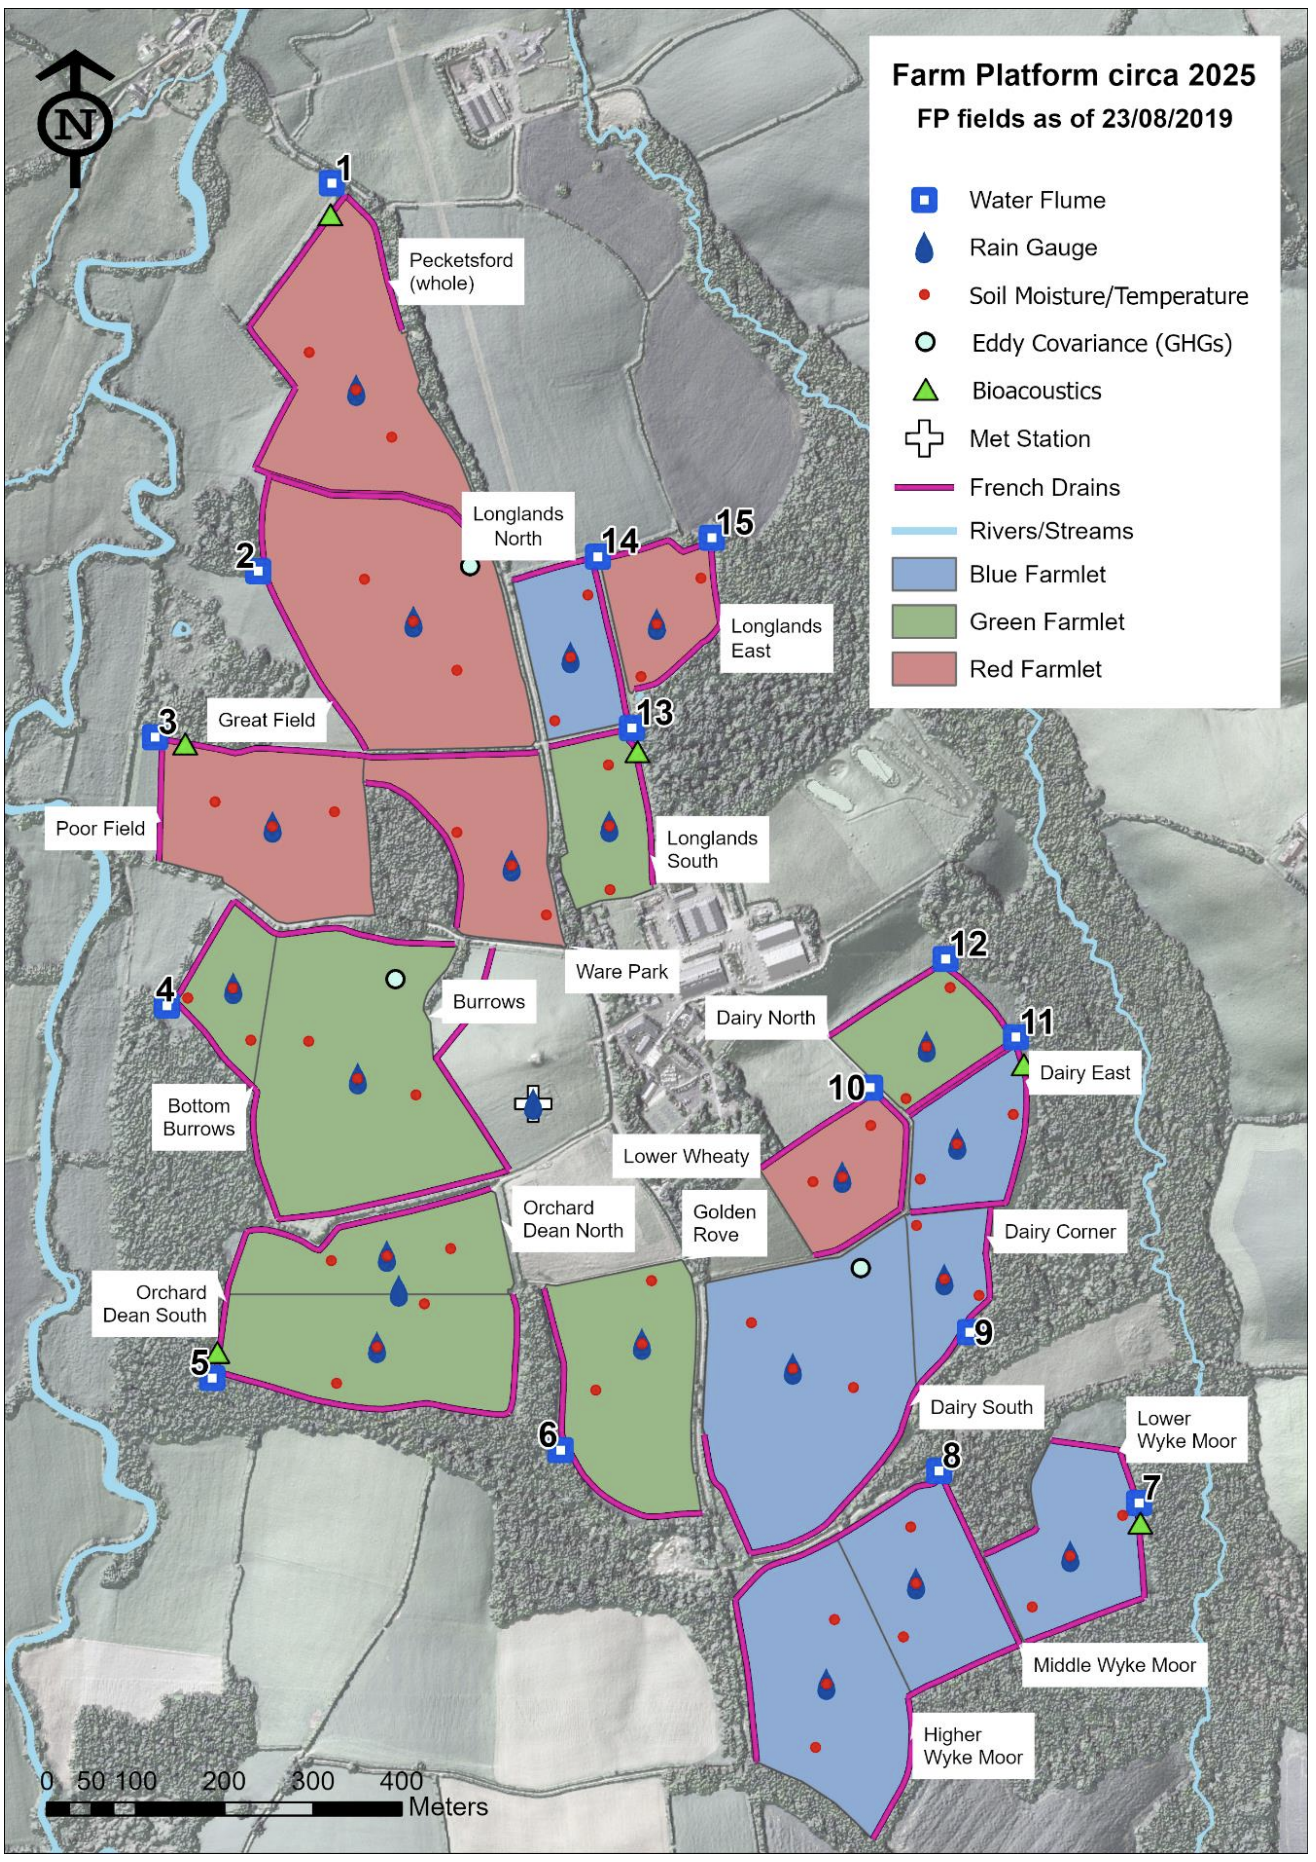
\includegraphics[
        width=0.82\textwidth,
        height=0.74\textheight,
        keepaspectratio
    ]{Figures/ch2_NWFP Map.png}
    \caption{Layout of the North Wyke Farm Platform circa 2025, showing the
    Red, Green, and Blue farmlets; The EC systems considered in this dissertation are
    situated in Great Field within Catchment~2, Burrows within Catchment~4,
    and Dairy South within Catchment~9. Cited from
    \cite{hawkins2023design}}
    \label{fig:nwfp-map}
\end{figure}

This dissertation examines measurements associated with three selected
catchments: Catchment~2 on the Red farmlet, Catchment~4 on the Green farmlet,
and Catchment~9 on the Blue farmlet, shown in
Figure~\ref{fig:nwfp-map}. These locations are denoted T2, T4, and T9
throughout the dissertation. The notation identifies the catchment containing
each EC site; it does not imply that NWFP comprises only three catchments.
Moreover, the three locations differ substantially in land use, vegetation,
livestock exposure, and measurement history. They should therefore be treated
as distinct modelling contexts rather than spatial replicates of a single
grassland treatment.

\begin{table}[htbp]
    \centering
    \small
    \caption{Characteristics of the NWFP catchments associated with the Eddy Covariance Towers.}
    \label{tab:nwfp-catchments}
    \begin{tabular}{
        @{}
        >{\raggedright\arraybackslash}p{0.07\textwidth}
        >{\raggedright\arraybackslash}p{0.19\textwidth}
        >{\raggedright\arraybackslash}p{0.35\textwidth}
        >{\raggedright\arraybackslash}p{0.30\textwidth}
        @{}
    }
        \toprule
        \textbf{Site} &
        \textbf{Location} &
        \textbf{Land use and management} &
        \textbf{Modelling significance} \\
        \midrule

        T2 &
        Catchment~2, Great Field, Red farmlet &
        Arable rotation including wheat, oats, and field beans. Great Field
        previously supported reseeded high-sugar perennial ryegrass, livestock
        grazing, and silage production. &
        Represents a pronounced grassland-to-arable transition rather than a
        continuously grazed pasture system. \\

        \addlinespace

        T4 &
        Catchment~4, Burrows, Green farmlet &
        Long-term permanent pasture managed through seasonal cattle and sheep
        grazing, silage production, inorganic fertiliser application, and the
        return of farmyard manure. &
        Represents the permanent-pasture system. Livestock presence within the
        EC footprint varies as animals rotate among fields. \\

        \addlinespace

        T9 &
        Catchment~9, Dairy South, Blue farmlet &
        High-sugar perennial ryegrass and white-clover pasture supporting
        cattle and sheep grazing and silage production, with biological nitrogen
        fixation reducing reliance on inorganic nitrogen fertiliser. &
        Represents the grass--clover livestock system, with temporally variable
        livestock presence and management activity. \\

        \bottomrule
    \end{tabular}
\end{table}

Together, T2, T4, and T9 represent three distinct combinations of land use,
vegetation, livestock exposure, and measurement availability. T2 captures a
grassland-to-arable transition, T4 represents long-term permanent pasture, and
T9 represents an established grass--clover livestock system. These differences
mean that observations from the three sites cannot be interpreted as spatial
replicates of a common management regime.

% ############################################################################
\subsection{Eddy Covariance Measurement and Flux Processing}

Eddy Covariance (EC) estimates the vertical exchange of a gas between the land
surface and atmosphere by combining rapid measurements of vertical wind velocity
with corresponding changes in gas concentration. In simplified form, the
turbulent flux of a gas \(c\) can be expressed as

\begin{equation}
    F_c = \overline{w'c'},
\end{equation}

where \(w'\) is the deviation of vertical wind velocity from its
averaging-period mean, \(c'\) is the corresponding deviation in gas
concentration, and the overbar denotes averaging through time. EC therefore
measures spatially integrated ecosystem exchange rather than emissions from an
individual source.

Each of the three EC systems identified in
Table~\ref{tab:nwfp-catchments} contains a Gill WindMaster Pro sonic anemometer
and an enclosed LI-7200RS analyser measuring carbon dioxide and water vapour.
Carbon-dioxide and water-vapour fluxes have been collected at all three systems
since January 2017. Two open-path LI-7700 analysers were subsequently deployed
for methane measurement from January 2018.

Because only two methane analysers were available, methane was not measured
continuously at all three locations. The analysers were initially installed at
T2 and T4 from January 2018 to June 2019. In July 2019, the analyser at T2 was
relocated to T9 following the conversion of the Red farmlet to arable
production. Consequently, T2 provides an earlier methane record from the Red
pasture system, T4 provides the most temporally consistent record, and T9
provides a later record from the Blue grass--clover system
\cite{olde2023ec}. These records are therefore neither continuous nor fully
contemporaneous.

Raw EC measurements are processed using EddyPro software, which calculates gas
fluxes and produces 30-minute averages recorded at the beginning and midpoint
of each hour. Timestamps are maintained in Coordinated Universal Time using the
analysers' GPS units. The resulting files follow the European Fluxes Database
format and retain quality flags, friction-velocity measurements, and footprint
information. Low-quality observations are not removed automatically and must
therefore be identified during data preparation \cite{olde2023ec}.

An EC observation represents a changing spatial footprint rather than a fixed
average of the field or catchment containing the system. The location and extent
of this footprint depend on wind direction, wind speed, atmospheric stability,
and measurement height, and may occasionally extend beyond the field boundary.
Recorded livestock presence at catchment level does not therefore guarantee that
the animals were inside the EC footprint at a particular timestamp. The
resulting FCH\textsubscript{4} measurement should be interpreted as integrated
methane exchange within this changing footprint.

This measurement scale also distinguishes EC from systems such as GreenFeed.
GreenFeed records methane released by an individual animal during discrete
visits, whereas EC integrates methane exchange associated with livestock,
manure, soil, vegetation, and other processes within its footprint
\cite{olde2023ec,demeofilho2023greenfeed}.

% ############################################################################
\subsection{EC Methane Gap-Filling and the Forecasting Gap}

EC records are rarely complete. Instrument maintenance, analyser servicing,
quality-control filtering, insufficient atmospheric turbulence, and periods in
which the estimated footprint falls outside the intended field can all remove
observations. At NWFP, these operational gaps coexist with the longer structural
absence created by relocating the methane analyser from T2 to T9. A continuous
historical FCH\textsubscript{4} series must therefore be constructed before flux
summaries and downstream forecasting models can be developed.

Zhu et al.\ provide the closest published same-site gap-filling comparison,
having evaluated MDS and machine-learning approaches using EC methane
measurements from the North Wyke managed pastures. All tested approaches
produced an OLS-regression \(R^2<0.10\) for FCH\textsubscript{4}: MDS achieved
approximately \(R^2=0.03\)--\(0.05\), while Random Forest performed relatively
better but remained below \(R^2=0.10\) \cite{zhu2023a}. These results establish
the difficulty of gap-filling methane flux at NWFP and provide the principal
published comparator for this dissertation. 

Evidence from other ecosystems generally supports the use of tree-based
methods. Irvin et al.\ found Random Forest and XGBoost to outperform neural and
linear models across 17 FLUXNET-CH4 wetland sites, although their uncertainty
estimates were systematically too narrow \cite{irvin2021}. Kim et al.\ similarly
reported strong Random Forest performance and found lagged environmental
variables particularly valuable for methane prediction \cite{kim2020}.
Nevertheless, these studies are dominated by wetlands and rice paddies rather
than managed livestock pasture. This motivates the same-site comparison of
established gap-filling methods, newer model families, and agricultural
management predictors undertaken in Chapter~\ref{Chap4}.

Importantly, these studies evaluate gap-filling rather than forecasting.
Gap-filling reconstructs missing observations within a historical record and
may use information from both before and after a gap. Forecasting instead
predicts beyond a defined forecast origin using only information available at
that point, with earlier predictions potentially becoming inputs during
recursive rollout. The published gap-filling results therefore establish a
relevant methodological baseline but do not demonstrate prospective predictive
skill. To the author's knowledge, no previous study has benchmarked multi-step
EC methane forecasting at a managed temperate grassland; this forms the second
modelling gap addressed by the dissertation.

% ############################################################################
\section{Advances in Tabular Machine Learning}
\label{sec:tabular-modelling}

Following temporal alignment and feature construction, the modelling tasks in
this dissertation take the form of supervised prediction over structured
tabular data. The candidate model families nevertheless differ substantially:
statistical models impose explicit temporal structure, tree ensembles learn
non-linear partitions from the study data, conventional deep-learning models
fit neural representations to the observed sequences, and tabular foundation
models transfer a prediction procedure learned through large-scale
pretraining. Two related questions therefore motivate the model roster used in
this dissertation: whether recent tabular foundation models transfer
effectively to EC methane data, and whether deep-learning methods outperform
established statistical and tree-based alternatives in this setting.

% ############################################################################
\subsection{Tabular Foundation Models}

Tabular foundation models are pretrained across many synthetic prediction tasks
and subsequently make predictions using labelled examples supplied as context.
The original TabPFN applied this approach to small classification problems,
while TabPFN v2 extended it to regression and larger tables
\cite{hollmann2023tabpfn,hollmann2025tabpfn}. TabPFN is not inherently a
time-series model, but Hoo et al.\ demonstrate that forecasting can be treated
as tabular regression by representing temporal position, seasonality, lags, and
other historical information as input features \cite{hoo2026tabpfnts}. This
formulation is directly relevant to the present dissertation, where EC methane
forecasting similarly uses calendar, environmental, management, and
autoregressive predictors.

TabICL was developed to extend in-context tabular learning to larger datasets
\cite{qu2025tabicl}. TabICLv2 subsequently introduced a redesigned
synthetic-data generator, more scalable attention, and revised pretraining
procedures, while supporting both regression and classification
\cite{qu2026tabiclv2}. Synthetic pretraining may be valuable at NWFP because
valid methane observations are limited, but general tabular benchmarks do not
establish performance under extensive missingness, non-stationarity, episodic
emission peaks, or recursive temporal extrapolation. The suitability of TabPFN
and TabICLv2 for EC methane modelling must therefore be determined through
task-specific evaluation.

% Tabular foundation models depart from conventional supervised learning by
% pretraining a neural model across many synthetic prediction tasks. The original
% TabPFN was trained to approximate Bayesian prediction over synthetically
% generated tabular datasets. At inference time, labelled training examples and
% unlabelled query examples are supplied together as context, allowing the model
% to generate predictions without conventional dataset-specific gradient-based
% training. The original implementation focused on small classification
% problems, while TabPFN v2 extended the approach to regression and larger
% tables \cite{hollmann2023tabpfn,hollmann2025tabpfn}. This combination of
% synthetic pretraining and in-context inference makes TabPFN potentially
% attractive where the available task-specific observations are limited.

% TabPFN is not inherently a time-series model. Hoo et al.\ address this by
% formulating forecasting as tabular regression: temporal position, seasonality,
% lags, and other historical information are represented as input features before
% inference with the pretrained TabPFN v2 model. Their TabPFN-TS approach
% therefore obtains forecasting capability without dedicated time-series
% pretraining \cite{hoo2026tabpfnts}. This formulation is directly relevant to
% the present dissertation, where EC methane forecasting is similarly represented
% using calendar, environmental, management, and autoregressive features.

% TabICL extends tabular in-context learning to larger datasets through an
% architecture designed to process features and observations more efficiently
% than earlier TabPFN implementations \cite{qu2025tabicl}. TabICLv2 subsequently
% extends this approach through a redesigned synthetic-data generator, more
% scalable attention, and revised pretraining procedures, while supporting both
% regression and classification \cite{qu2026tabiclv2}. Its relevance to this
% dissertation lies in the possibility that knowledge acquired during synthetic
% pretraining may compensate for the limited number of valid methane
% observations available at NWFP.

% Strong performance on general tabular benchmarks does not, however, guarantee
% successful transfer to EC methane modelling. NWFP combines extensive target
% missingness, heterogeneous environmental and management predictors,
% non-stationary land-management conditions, and a highly variable target
% containing episodic emission peaks. Forecasting also introduces temporal
% extrapolation and recursive error propagation that are absent from ordinary
% independent tabular regression. TabPFN and TabICLv2 must therefore be evaluated
% under the same task-specific temporal protocol as the other model families
% rather than assumed to be superior on the basis of their published benchmarks.

% ############################################################################
\subsection{Deep Learning versus Traditional Machine Learning}

Large tabular benchmarks do not establish universal superiority of deep
learning. Grinsztajn et al.\ compared tree ensembles and neural architectures
across 45 medium-sized datasets and found tree-based models to remain
state-of-the-art, attributing this partly to their robustness to uninformative
features and irregular response functions \cite{grinsztajn2022}. McElfresh
et al.\ reached a more conditional conclusion from 19 algorithms and 176
datasets: neural and boosted-tree performance was often similar, modest
boosted-tree tuning could matter more than model-family choice, and relative
performance depended strongly on dataset characteristics
\cite{mcelfresh2023}. This pattern is consistent with EC methane studies, in
which Random Forest and XGBoost have generally provided stronger baselines than
conventional neural alternatives \cite{irvin2021,kim2020,zhu2023a}. These
findings justify retaining tree ensembles as serious comparators without
assuming that they must remain superior when richer predictors or pretrained
models are introduced.

A comparable debate exists in time-series forecasting. Zeng et al.\ found that
simple one-layer linear models outperformed several Transformer architectures
across nine long-term forecasting datasets \cite{zeng2023}. This does not imply
that complex architectures are universally ineffective, but demonstrates that
architectural sophistication cannot itself be treated as evidence of predictive
skill. Tabular foundation models further complicate the comparison: TabPFN and
TabICLv2 are neural models, but their capabilities are largely acquired through
pretraining rather than learned exclusively from the study dataset. The
relevant empirical comparison is therefore among statistical baselines, tree
ensembles, locally trained deep-learning models, and pretrained tabular
foundation models under identical evaluation conditions.

% ############################################################################
\section{Synthesis and Gap Statement}

Existing research demonstrates that machine learning can reconstruct missing
EC methane observations, but the closest North Wyke comparison reports weak
predictive performance, and the wider evidence is dominated by wetlands and
rice paddies, not grassland farming. Moreover, these studies evaluate gap-filling 
within historical records rather than multi-step forecasting beyond a defined 
forecast origin. To the author's knowledge, no previous study has benchmarked 
methane flux forecasting at a managed temperate grassland.

Recent TabPFN and TabICL models have also not been evaluated for this
combination of ecosystem, measurement type, and prediction tasks. It therefore
remains unknown whether synthetic pretraining provides an advantage over
established statistical, tree-based, and conventional deep-learning approaches
under severe target missingness and temporal extrapolation. This dissertation
addresses these gaps by comparing the model families under common,
leakage-safe gap-filling and forecasting protocols, accompanied by uncertainty
quantification and interpretability. The resulting forecasting architecture is
then applied to bounded scenario projection under contrasting management and
climate conditions.

% Existing evidence does not establish a universally superior model family for
% structured environmental prediction. Large tabular benchmarks show that tree
% ensembles remain highly competitive, particularly for medium-sized and
% irregular datasets, but also demonstrate that the relative performance of
% neural and tree-based models depends on dataset characteristics and tuning
% \cite{grinsztajn2022,mcelfresh2023}. Meanwhile, the recent TabPFN and TabICL
% families have not been evaluated for EC methane gap-filling and multi-step
% forecasting at a managed temperate grassland. Whether synthetic pretraining
% offers an advantage under severe missingness, temporal extrapolation, and
% episodic methane behaviour therefore remains unresolved and presents an 
% opportunity for investigation within this dissertation.
